%----------------------------------------------------------------------------------------
%	PACKAGES AND OTHER DOCUMENT CONFIGURATIONS
%----------------------------------------------------------------------------------------

\documentclass[11pt]{scrartcl} % Font size

%%%%%%%%%%%%%%%%%%%%%%%%%%%%%%%%%%%%%%%%%
% Wenneker Assignment
% Structure Specification File
% Version 2.0 (12/1/2019)
%
% This template originates from:
% http://www.LaTeXTemplates.com
%
% Authors:
% Vel (vel@LaTeXTemplates.com)
% Frits Wenneker
%
% License:
% CC BY-NC-SA 3.0 (http://creativecommons.org/licenses/by-nc-sa/3.0/)
% 
%%%%%%%%%%%%%%%%%%%%%%%%%%%%%%%%%%%%%%%%%

%----------------------------------------------------------------------------------------
%	PACKAGES AND OTHER DOCUMENT CONFIGURATIONS
%----------------------------------------------------------------------------------------

\usepackage{amsmath, amsfonts, amsthm} % Math packages

\usepackage{listings} % Code listings, with syntax highlighting

\usepackage{graphicx} % Required for inserting images

\usepackage{booktabs} % Required for better horizontal rules in tables

\usepackage{dirtytalk} % Required for quoting.

\usepackage{float} % Added for hard placement of images.

\usepackage[dvipsnames]{xcolor} % Added for extra colors.

\usepackage{tikz} % For colored boxes and more.

\numberwithin{equation}{section} % Number equations within sections (i.e. 1.1, 1.2, 2.1, 2.2 instead of 1, 2, 3, 4)
\numberwithin{figure}{section} % Number figures within sections (i.e. 1.1, 1.2, 2.1, 2.2 instead of 1, 2, 3, 4)
\numberwithin{table}{section} % Number tables within sections (i.e. 1.1, 1.2, 2.1, 2.2 instead of 1, 2, 3, 4)

\usepackage{enumitem} % Required for list customisation
\setlist{noitemsep} % No spacing between list items

\usepackage[main=greek, english]{babel}

%----------------------------------------------------------------------------------------
%	DOCUMENT MARGINS
%----------------------------------------------------------------------------------------

\usepackage{geometry} % Required for adjusting page dimensions and margins

\geometry{
	paper=a4paper, % Paper size, change to letterpaper for US letter size
	top=2.5cm, % Top margin
	bottom=3cm, % Bottom margin
	left=3cm, % Left margin
	right=3cm, % Right margin
	headheight=0.75cm, % Header height
	footskip=1.5cm, % Space from the bottom margin to the baseline of the footer
	headsep=0.75cm, % Space from the top margin to the baseline of the header
	%showframe, % Uncomment to show how the type block is set on the page
}

%----------------------------------------------------------------------------------------
%	FONTS
%----------------------------------------------------------------------------------------

\usepackage[utf8]{inputenc} % Required for inputting international characters
\usepackage[T1]{fontenc} % Output font encoding for international characters

\usepackage{XCharter} % Use the XCharter fonts


%----------------------------------------------------------------------------------------
%	SECTION TITLES
%----------------------------------------------------------------------------------------

\usepackage{sectsty} % Allows customising section commands

\sectionfont{\vspace{6pt}\centering\normalfont\scshape} % \section{} styling
\subsectionfont{\normalfont\bfseries} % \subsection{} styling
\subsubsectionfont{\normalfont\itshape} % \subsubsection{} styling
\paragraphfont{\normalfont\scshape} % \paragraph{} styling

%----------------------------------------------------------------------------------------
%	HEADERS AND FOOTERS
%----------------------------------------------------------------------------------------

\usepackage{scrlayer-scrpage} % Required for customising headers and footers

\ohead*{} % Right header
\ihead*{} % Left header
\chead*{} % Centre header

\ofoot*{} % Right footer
\ifoot*{} % Left footer
\cfoot*{\pagemark} % Centre footer

\newcommand{\img}[1] % maybe add a caption to this
{
    \begin{center}
        \fcolorbox{black}{white}{\includegraphics[width=\textwidth]{#1}}
    \end{center}

}

% Helper Macros

\newcommand{\en}[1]{\foreignlanguage{english}{#1}}
\newcommand{\src}[1]{{\texttt{#1}}}


% Extra Formatting

\setlength{\parindent}{0em}
\setlength{\parskip}{0em}


% Code Listing Style

\lstdefinestyle{code}{
  belowcaptionskip=1\baselineskip,
  breaklines=true,
  frame=LRTB,
  xleftmargin=\parindent,
  showstringspaces=false,
  basicstyle=\ttfamily,
  keywordstyle=\bfseries\color{green!40!black},
  commentstyle=\itshape\color{purple!40!black},
  identifierstyle=\color{black},
  stringstyle=\color{orange},
}


\newcommand{\lstcode}[3]
{
    \begin{otherlanguage}{english}
    \lstinputlisting[language=#2, frame=single, style=code, caption=#3]{#1}
    \end{otherlanguage}
}
 % Include the file specifying the document structure and custom commands
\usepackage{multirow}
\usepackage{array}
\usepackage{subcaption}
% Bar chart drawing library 
\usepackage{pgfplots} 
\usepackage{textcomp}
\usepackage{algorithm}
\usepackage{algpseudocode}

\usetikzlibrary{positioning}

% Define a macro to create a table with fixed column widths
\newcolumntype{C}[1]{>{\centering\arraybackslash}p{#1}}

\usepackage{hyperref}
\hypersetup{
    colorlinks=true,
    linkcolor=blue,
    filecolor=magenta,      
    urlcolor=cyan,
}

\definecolor{diffstart}{named}{Apricot}
\definecolor{diffincl}{named}{Green}
\definecolor{diffrem}{named}{Red}

\usepackage{listings}
  \lstdefinelanguage{diff}{
    basicstyle=\ttfamily\small,
    morecomment=[f][\color{diffstart}]{@@},
    morecomment=[f][\color{diffincl}]{+\ },
    morecomment=[f][\color{diffrem}]{-\ },
  }

\definecolor{codegreen}{rgb}{0,0.6,0}
\definecolor{codegray}{rgb}{0.5,0.5,0.5}
\definecolor{codepurple}{rgb}{0.58,0,0.82}
\definecolor{backcolour}{rgb}{0.95,0.95,0.92}
\definecolor{codeblue}{rgb}{0,0,0.8}

\lstdefinestyle{mystyle}{
    backgroundcolor=\color{backcolour},   
    commentstyle=\color{codegreen},
    keywordstyle=\color{codeblue},
    numberstyle=\tiny\color{codegray},
    stringstyle=\color{codepurple},
    basicstyle=\ttfamily\footnotesize,
    breakatwhitespace=false,         
    breaklines=true,                 
    captionpos=b,                    
    keepspaces=true,                 
    numbers=left,                    
    numbersep=5pt,                  
    showspaces=false,                
    showstringspaces=false,
    showtabs=false,                  
    tabsize=2
}
\usepackage{tocloft}
\renewcommand{\cftsecfont}{\normalfont}
\renewcommand{\cftsecpagefont}{\normalfont}
\addto\captionsgreek{\renewcommand{\contentsname}{\normalfont Περιεχόμενα}}

\lstset{style=mystyle}

%----------------------------------------------------------------------------------------
%	TITLE SECTION
%----------------------------------------------------------------------------------------

\title{	
	\normalfont\normalsize
	\textsc{Πανεπιστήμιο Πατρών, Τμήμα Μηχανικών ΗΥ και Πληροφορικής}\\ % Your university, school and/or department name(s)
	\vspace{25pt} % Whitespace
	\rule{\linewidth}{0.5pt}\\ % Thin top horizontal rule
	\vspace{20pt} % Whitespace
    {\Large Λογισμικό και Προγραμματισμός Συστημάτων Υψηλής Επίδοσης \\ \textbf{Final Project:} Function approximation with k-Nearest Neighbors}\\ % The assignment title
	\vspace{12pt} % Whitespace
	\rule{\linewidth}{2pt}\\ % Thick bottom horizontal rule
	\vspace{12pt} % Whitespace
}

\author{Ευάγγελος Λάμπρου \\UP1066519 \and Ιωάννης Παναρίτης \\UP1072632} % Your name

\date{} % Today's date (\today) or a custom date

%----------------------------------------------------------------------------------------
%	DOCUMENT
%----------------------------------------------------------------------------------------

\bibliographystyle{ieeetr}
\addto\captionsgreek{\renewcommand{\refname}{Αναφορές}}


\begin{document}

\maketitle 
\tableofcontents

\section{Εισαγωγή}

Στην εργασία αυτή σκοπός είναι η επιτάχυνση ενός προγράμματος, το οποίο
δοθέντος ενός συνόλου σημείων $x$ και της αντίστοιχης τιμής $y = f(x)$ (για οποιαδήποτε συνάρτηση $f$), 
θα είναι σε θέση, δοθέντος ενός νέου σημείο $x'$ θα μπορεί να προβλέψει, με τη χρήση του αλγορίθμου 
k-Nearest Neighbors (KNN) την αντίστοιχη τιμή $y'$.

Η συνάρτηση με βάση την οποία παράγουμε τα σημεία είναι η 16-διάστατη συνάρτηση \say{κύκλου}.

Σε όλες τις μετρήσεις, ετκός και αν επισημαίνεται διαφορετικά, χρησιμοποιούμε μηχάνημα με τα εξής χαρακτηριστικά:
\begin{itemize}
    \item Επεξεργαστής: \src{Intel(R) Core(TM) i7-3770K CPU @ 3.50GHz}
    \item Κάρτα Γραφικών: \src{NVIDIA Corporation GK180GL [Tesla K40c]}
\end{itemize}

\section{Υλοποιήσεις}

\subsection{Σειριακή}

\subsubsection{Αρχική Υλοποίηση}

Στη σειριακή υλοποίηση το πρόγραμμα αποτελείται από τρία μέρη: 

\begin{enumerate}
    \item Φόρτωση των δεδομένων εκπαίδευσης (training) και ερωτήσεων (query).
    \item Εκτέλεση του αλγορίθμου KNN για κάθε ένα από τα σημεία ερώτησης.
    \item Παρουσίαση των αποτελεσμάτων (APE, MSE, $R^2$, χρόνοι εκτέλεσης)
\end{enumerate}

Για τον υπολογισμό του κάθε σημείου, ο KNN λειτουργεί ως εξής:

\begin{enumerate}
    \item Υπολογισμός της απόστασης του σημείου ερώτησης (query point) με όλα τα σημεία εκπαίδευσης.
    \item Επιλογή των $k$ σημείων με τη χαμηλότερη απόσταση από το query point. (γίνεται sorting πάνω στον πίνακα των αποστάσεων)
    \item Πρόβλεψη της τιμής του σημείου ερώτησης με βάση τις τιμές των $k$ επιλεγμένων σημείων. (μέσος όρος, weighted average, κλπ)
\end{enumerate}

Εκτελώντας την σειριακή υλοποίηση από τον perf profiler έχουμε τα ακόλουθα αποτελέσματα:

\lstinputlisting[caption={Αποτελέσματα του \src{perf report x.txt q.txt} (χωρίς τις κλήσεις στη βασική βιβλιοθήκη C)}, label={lst:perf}]{./assets/report-serial.txt}

Φαίνεται πως το μεγαλύτερο ποσοστό του χρόνου βρίσκεται στις συναρτήσεις \src{compute\_max\_pos} και \src{compute\_dist}, οι οποίες με τη σειρά τους εκτελούνται 
μέσα από την \src{compute\_knn\_brute\_force}. Συνεπώς, στόχος μας είναι η παραλληλοποίηση του \src{compute\_knn\_brute\_force}.

\subsubsection{Διαχείριση των δεδομένων}

Στην αρχική υλοποίηση του πργράμματος για κάθε query διαβαζόταν το επόμενο σημείο από το αρχείο \src{q.txt}. 
Ωστόσο, αυτό έχει ως αποτέλεσμα την δυσκολία παραλληλοποίησης του υπολογισμού των queries (δηλαδή το να υπολογίζονται πολλά queries ταυτόχρονα).
Έτσι, μετατρέπουμε το αρχείο \src{q.txt} σε έναν πίνακα στη μνήμη, ώστε να μπορούμε να προσπελάσουμε τα σημεία ερώτησης με την σειριακή σειρά που έχουν στο αρχείο.
Τελικά, έχουμε την επιλογή είτε να υλοποιήσουμε τα βήματα του αλγορίθμου KNN, ή να τρέχουμε πολλούς ξεχωριστούς αλγορίθμους KNN παράλληλα.

% create a figure with two subfigures
% the first subfigure should be the diagram you created above
% the second subfigure should be empty
% the two subfigures should be side by side
% the two subfigures should be centered in the page
\begin{figure}[H]
    \centering
    \begin{subfigure}[t]{0.4\textwidth}
        \centering
        \begin{tikzpicture}
            \node [draw, minimum width=15em, minimum height=15em, label=above:Program] (program) at (0,0) {};
            \node [draw, fill=blue!20, minimum width=1cm, minimum height=1cm] (query1) at (0, 2)  {k-NN query};
            \node [draw, fill=blue!20, minimum width=1cm, minimum height=1cm, below=.3cm of query1] (query2)  {k-NN query};
            \node [draw, fill=blue!20, minimum width=1cm, minimum height=1cm, below=.3cm of query2] (query3)  {k-NN query};
            \node [draw, fill=blue!20, minimum width=1cm, minimum height=1cm, below=.3cm of query3] (query4)  {k-NN query};

            \draw [decorate, decoration = {brace, amplitude=5pt}] (query1.north east) -- (query4.south east)  node [midway, label=right:Parallel] {};
        \end{tikzpicture}
        \caption{Παραλληλοποίηση επιπέδου query.}
    \end{subfigure}
    \begin{subfigure}[t]{0.4\textwidth}
        \centering
        \begin{tikzpicture}
            \node [draw, minimum width=15em, minimum height=15em, label=above:Program] (program) at (0,0) {};
            \node [draw, fill=blue!20, minimum width=5cm, minimum height=4cm, label=above:k-NN query] (KNN) at (0, 0)  {};
            % draw 3 red rectangles inside the blue rectangle
            \node [draw, fill=red!20, minimum width=4cm, minimum height=.5cm, below=.3cm of KNN.north] (point1) {\src{compute\_distance}};
            \node [draw, fill=red!20, minimum width=4cm, minimum height=.5cm, below=.3cm of point1] (point2)  {\src{compute\_distance}};
            \node [draw, fill=red!20, minimum width=4cm, minimum height=.5cm, below=.3cm of point2] (point3)  {\src{compute\_distance}};
            \node [draw, fill=red!20, minimum width=4cm, minimum height=.5cm, below=.3cm of point3] (point4)  {...};

            \draw [decorate, decoration = {brace, amplitude=5pt}] (point1.north east) -- (point4.south east)  node [midway, label=right:Parallel] {};
        \end{tikzpicture}
        \caption{Παραλληλοποίηση του αλγορίθμου KNN}
    \end{subfigure}
    \caption{Παραλληλοποίηση του της εφαρμογής σε επίπεδο query και σε επίπεδο αλγορίθμου}
\end{figure}

\subsubsection{Αλγόριθμος Ταξινόμησης}

Για την επιλογή των $k$ κοντινότερων σημείων πρέπει στην ουσία να
ταξινομήσουμε τις αποστάσεις και να επιλέξουμε τα πρώτα $k$ σημεία.
Ωστόσο, έτσι όπως είναι υλοποιημένη η ρουτίνα που υπολογίζει τις αποστάσεις και
τοποθετεί τιμές αποστάσεων και indexes στους πίνακες \src{nn\_d} και \src{nn\_x} αντίστοιχα, 
στην ουσία έχουμε στα χέρια μας ήδη τα $k$ κοντινότερα σημεία, απλά δεν είναι με αύξουσα σειρά απόστασης.
Αυτό βέβαια δεν έχει σημασία για το τελικό αποτέλεσμα.
Συνεπώς, μπορούμε να αφαιρέσουμε ολοκλληρωτικά τη ρουτίνα ταξινόμησης.

Αρχικά είχαμε δοκιμάσει να χρησιμοποιήσουμε τον αλγόριθμο merge sort \cite{mergesort} 
αξιοποιώντας την παραλληλίσιμη φύση του.
Ωστόσο, οι μετρήσεις ταχύτητας έδειξαν πως δεν υπήρχε βελτίωση διότι ο πίνακας 
τον οποίο ταξινομούμε είναι πολύ μικρός σε μέγεθος ($k$ στοιχεία).

\subsubsection{Αναδιάταξη Πράξεων}

\begin{itemize}

    \item Παρατηρώντας τα αποτελέσματα του profiler, βλέπουμε πως αφιερώνεται αρκετός χρόνος στη συνάρτηση \src{compute\_max\_pos}.
Έτσι, αναλύοντας τον κώδικα παρατηρήσαμε πως η συνάρτηση αυτή χρησιμοποιείται στη συνάρτηση \src{compute\_distance} σε μεγαλύτερο 
βαθμό απ'ότι χρειάζεται.

\lstinputlisting[language=diff]{./assets/compute_max.c.diff}

Είναι προφανές, ότι το index για το πού πρέπει να τοποθετηθεί το εκάστοτε σημείο στο array δεν χρειάζεται να υπολογίζεται σε 
κάθε επανάληψη, παρά μόνο τις φορές όπου υπάρχει υποψήφιο νέο σημείο με κοντινότερη απόσταση.
Αυτή η \say{διόρθωση} δίνει σοβαρή επιτάχυνση στη σειριακή υλοποίηση.

    \item Ακόμα, το ίδιο loop είναι υπεύθυνο για τον υπολογισμό των αποστάσεων μεταξύ 
        του query point και των υπόλοιπων σημείων.
        Έτσι, χωρίσαμε το μέρος του loop το οποίο υπολογίζει την απόσταση των σημείων 
        και τα αποθηκεύουμε σε έναν ενδιάμεσο πίνακα (\src{d\_dist}). 
        Στην συνέχεια αναφερόμαστε στην απόσταση του σημείου $q$ με το σημείο $i$
        ώς \src{d\_dist[i]}.

\lstinputlisting[language=diff]{./assets/dist.c.diff}

\end{itemize}

\subsubsection{Υπολογισμός Απόστασης}

Για την σύγκριση της απόστασης μεταξύ δύο σημείων ισχύει:

\begin{equation}
    \begin{split}
        dist(x_1, q) < dist(x_2, q) &= \\
        \sqrt{(x_{11} - q_1)^2 + (x_{12} - q_2)^2} < \sqrt{(x_{21} - q_1)^2 + (x_{22} - q_2)^2} &= \\
        {(x_{11} - q_1)^2 + (x_{12} - q_2)^2} < {(x_{21} - q_1)^2 + (x_{22} - q_2)^2}
    \end{split}
\end{equation}

Συνεπώς, για τον υπολογισμό της απόστασης, εφόσον ο αλγόριθμός μας
βασίζεται μόνο στη σύγκριση μεταξύ των αποστάσεων και όχι στις ακριβείς τιμές τους, μπορούμε 
να αποφύγουμε τη συνάρτηση \src{sqrt} στον υπολογισμό της απόστασης. 
Αυτό δίνει μία μικρή βελτίωση στο χρόνο εκτέλεσης.

\subsubsection{Inverse Weight Average}

Τέλος, για την πρόβλεψη της νέας τιμής για το κάθε σημείο με βάση τα $k$ κοντινότερα 
σημεία, ανταλλάξαμε την αρχική υλοποίηση που υπολόγιζε την μέση τιμή (mean) της τιμής 
της συνάρτησης στα $k$ σημεία, με τη μετρική inverse distance weight.

\subsubsection{Μετρήσεις}

\begin{figure}[H]
    \begin{center}
\begin{tikzpicture}
    \begin{axis}[
        xlabel={Αριθμός Queries},
        ylabel={Χρόνος/Query (ms)},
        xtick=data,
        xticklabels={32, 1024},
        ybar,
        enlarge x limits=0.15,
        bar width=10pt,
        legend style={at={(0.5,-0.20)}, anchor=north, legend columns=-1},
        legend entries={Πριν, Βελτιωμένο},
        ymajorgrids=true,
        y grid style=dashed,
        nodes near coords,
        nodes near coords align={vertical},
        nodes near coords style={anchor=north},
        every node near coord/.append style={yshift=-2pt},
        every axis plot post/.append style={fill=blue!20},
        ]
        \addplot coordinates {(1024, 41)};
        \addplot coordinates {(1024, 10)};
    \end{axis}
\end{tikzpicture}
    \end{center}
    \caption{Συνολικός χρόνος εκτέλεσης/query της σειριακής υλοποίησης πριν και μετά τις βελτιώσεις.}
    \label{fig:before_after_times}
\end{figure}

\subsection{Alternative Υλοποίηση}
Για αποδοτικότερο και πιο γρήγορο υπολογισμό δημιουργήθηκε μια διαφορετική υλοποίηση. Σε αυτήν έχουμε υπολογισμό των distances όλων των query,
και ύστερα πραγματοποίηση των επόμενων βημάτων. Αυτό θα μας δώσει την δυνατότητα να παραλληλοποιήσουμε σε μεγαλύτερο βαθμό τον knn, με
trade-off ότι χρειαζόμαστε αρκετή μνήμη για να αποθηκεύσουμε το μητρώο dist.

\subsection{OpenMP}

Στην OpenMP υλοποίηση του προγράμματος, αρχικά χρησιμοποιήσαμε μερικά OMP directives
για να επιταχύνουμε μερικές από τις ρουτίνες του αλγορίθμου ΚΝΝ.
Ωστόσο, παρατηρώντας ότι η πλειοψηφία των loops τρέχουν για λίγες επαναλήψεις, δεν πετύχαμε σημαντική επιτάχυνση στο χρόνο ανά query.
Παραλληλοποιώντας όμως σε επίπεδο query, είχαμε μια σημαντική επιτάχυνση στο συνολικό χρόνο εκτέλεσης του προγράμματος.

\subsubsection{Μετρήσεις}

\begin{figure}[H]
    \begin{center}
        \begin{subfigure}[b]{0.5\textwidth}
\begin{tikzpicture}
    \begin{axis}[
        xlabel={Αριθμός Threads},
        ylabel={Time/Query (ms)},
        xtick=data,
        xticklabels={2, 3, 4, 5, 6, 7, 8},
        enlarge x limits=0.15,
        bar width=10pt,
        ymajorgrids=true,
        y grid style=dashed,
        nodes near coords,
        nodes near coords align={vertical},
        nodes near coords style={anchor=north},
        every node near coord/.append style={yshift=-2pt},
        ]
        \addplot coordinates {(2, 9.60) (3, 5.56) (4, 7.36) (5, 6.69) (6, 4.75) (7, 4.18) (8, 3.55)};
    \end{axis}
\end{tikzpicture}
            \caption{Time}
        \end{subfigure}
        \begin{subfigure}[b]{0.5\textwidth}
\begin{tikzpicture}
    \begin{axis}[
        xlabel={Αριθμός Threads},
        ylabel={Time/Query Speedup},
        xtick=data,
        xticklabels={2, 3, 4, 5, 6, 7, 8},
        enlarge x limits=0.15,
        bar width=10pt,
        ymajorgrids=true,
        y grid style=dashed,
        nodes near coords,
        nodes near coords align={vertical},
        nodes near coords style={anchor=north},
        every node near coord/.append style={},
        ]
        \addplot coordinates {(2 ,1.04) (3 ,1.79) (4 ,1.35) (5 ,1.49) (6 ,2.10) (7 ,2.38) (8 ,2.80)};
    \end{axis}
\end{tikzpicture}
            \caption{Speedup}
        \end{subfigure}
    \end{center}
    \caption{Μετρήσεις για την υλοποίηση OMP}
    \label{fig:omp}
\end{figure}



\subsection{OpenACC}

Για την υλοποίηση με OpenACC κάναμε προσέγγιση παρόμοια με αυτή της OpenMP, δηλαδή
παραλληλοποιήσαμε ρουτίνες του αλγορίθμου KNN. 
Βασική διαφορά τώρα όμως είναι πως προκειμένου να δούμε μείωση στο συνολικό χρόνο εκτέλεσης έπρεπε 
να ελαχιστοποιήσουμε τις μεταφορές δεδομένων μεταξύ επεξεργαστή και κάρτας γραφικών.

\subsubsection{Μετρήσεις}

\begin{figure}[H]
    \begin{center}
\begin{tikzpicture}
    \begin{axis}[
        xlabel={Αριθμός Queries},
        ylabel={Time (ms)},
        xtick=data,
        xticklabels={1024},
        ybar,
        enlarge x limits=0.15,
        bar width=10pt,
        legend style={at={(0.5,-0.20)}, anchor=north, legend columns=-1},
        legend entries={Serial, OpenACC},
        ymajorgrids=true,
        y grid style=dashed,
        nodes near coords,
        nodes near coords align={vertical},
        nodes near coords style={anchor=north},
        every node near coord/.append style={yshift=-2pt},
        every axis plot post/.append style={fill=blue!20},
        ]
        \addplot coordinates {(1024, 10)};
        \addplot coordinates {(1024, 6.69)};
    \end{axis}
\end{tikzpicture}
    \end{center}
    \caption{Χρόνος εκτέλεσης/query}
    \label{fig:cluster_times}
\end{figure}

Έχουμε ένα τελικό speedup της τάξης του \textbf{1.5x}.

\subsection{CUDA}

Για την υλοποίηση με CUDA ουσιαστικά επιταχύνουμε την ρουτίνα υπολογισμού της απόστασης του σημείου
query με όλα τα άλλα σημεία.
Ορίζουμε ένα kernel \src{compute\_dist} το οποίο υπολογίζει την απόσταση του σημείου query με όλα τα άλλα σημεία 
και αποθηκεύει τα αποτελέσματα σε ένα array.

\subsubsection{Μετρήσεις}

\begin{figure}[H]
    \begin{center}
        \begin{subfigure}[b]{0.5\textwidth}
\begin{tikzpicture}
    \begin{axis}[
        xlabel={Αριθμός Threads/Block},
        ylabel={Time/Query (ms)},
        xtick=data,
        xticklabels={32, 64, 128, 256},
        enlarge x limits=0.15,
        bar width=10pt,
        ymajorgrids=true,
        y grid style=dashed,
        nodes near coords,
        nodes near coords align={vertical},
        nodes near coords style={anchor=north},
        every node near coord/.append style={yshift=-2pt},
        ]
        \addplot coordinates {(32, 2.59) (64, 2.59) (128, 2.59) (256, 2.59)};
    \end{axis}
\end{tikzpicture}
            \caption{Time}
        \end{subfigure}
        \begin{subfigure}[b]{0.5\textwidth}
\begin{tikzpicture}
    \begin{axis}[
        xlabel={Αριθμός Threads/Block},
        ylabel={Time/Query Speedup},
        xtick=data,
        xticklabels={32, 64, 128, 256},
        enlarge x limits=0.15,
        bar width=10pt,
        ymajorgrids=true,
        y grid style=dashed,
        nodes near coords,
        nodes near coords align={vertical},
        nodes near coords style={anchor=north},
        every node near coord/.append style={},
        ]
        \addplot coordinates {(32, 3.89) (64, 3.89) (128, 3.89) (256, 3.89)};
    \end{axis}
\end{tikzpicture}
            \caption{Speedup}
        \end{subfigure}
    \end{center}
    \caption{Μετρήσεις για την υλοποίηση CUDA}
    \label{fig:cuda}
\end{figure}

Το τελικό speedup είναι της τάξης του \textbf{3.89x}.
Παρατηρούμε πως ο αριθμός των threads/block δεν επηρεάζει τον χρόνο εκτέλεσης.


\subsection{MPI}

Για την υλοποίηση με MPI αποφασίσαμε να παραλληλοποιήσουμε τα ίδια τα queries και όχι το κάθε query ξεχωριστά, 
ουσιαστικά το κάθε process θα εκτελεί όλα τα queries που του αντιστοιχούν.
Αυτό έγινε για να ελαχιστοποιήσουμε τις μεταφορές δεδομένων μεταξύ των διεργασιών, αφού δεν θα υπάρχει ανταλλαγή δεδομένων παρά μόνο στην εκκίνηση και στη λήξη του αλγορίθμου.

Η λύση στην οποία καταλήξαμε έχει το μειονέκτημα ότι πρέπει ολόκληρο το training dataset να είναι παρών σε καθένα από 
τους MPI κόμβους.

Μια εναλλακτική προσέγγιση θα ήταν ο διαχωρισμός του πίνακα \src{x\_data}, έτσι ώστε σε κάθε query
να γινόταν παράλληλα ο υπολογισμός απόστασης του σημείου \src{q} με το κάθε σημείο ενός υποσύνολου του training set.

\subsubsection{MPI Cluster και OpenMP}

Επόμενος στόχος ήταν η δημιουργία ενός MPI cluster, όπου θα είχαμε παραπάνω από ένα μηχάνημα μέσα σε περιβάλλον LAN να εκτελούν τα queries.

Οι διεργασίες που εκτελούνται στον κάθε cluster μπορούν να παραλληλοποιηθούν περαιτέρω.
Έτσι, αφού είχαμε τη βασική υλοποίηση με MPI, προσθέσαμε στον κώδικα παραλληλοποίηση με OpenMP στον κώδικα του αλγορίθμου k-NN.

Τα βήματα για να δημιουργήσουμε ένα MPI cluster είναι τα εξής:

\begin{enumerate}
\item Εγκατάσταση του MPI σε όλα τα μηχανήματα.
\item Εγκατάσταση του OpenMPI σε όλα τα μηχανήματα.
\item Εγκατάσταση του OpenSSH σε όλα τα μηχανήματα, ενεργοποίηση του SSH server και δημιουργία κατάλληλων ssh κλειδιών.
\item Εγκατάσταση του NFS \cite{nfs} σε όλα τα μηχανήματα, ενεργοποίηση του NFS server και
        δημιουργία κοινόχρηστου φακέλου. Εκεί θα βρίσκεται το εκτελέσιμο και τα
        δεδομένα που θα χρησιμοποιούνται.
\item Εκτέλεση του κώδικα στον κύριο κόμβο με την εντολή:
\begin{lstlisting}
mpirun -np 6 --host laptop:1,desktop:4,ioanna:1 ./myknn-mpi x.txt q.txt
\end{lstlisting}
\end{enumerate}

\begin{figure}
    \begin{center}
        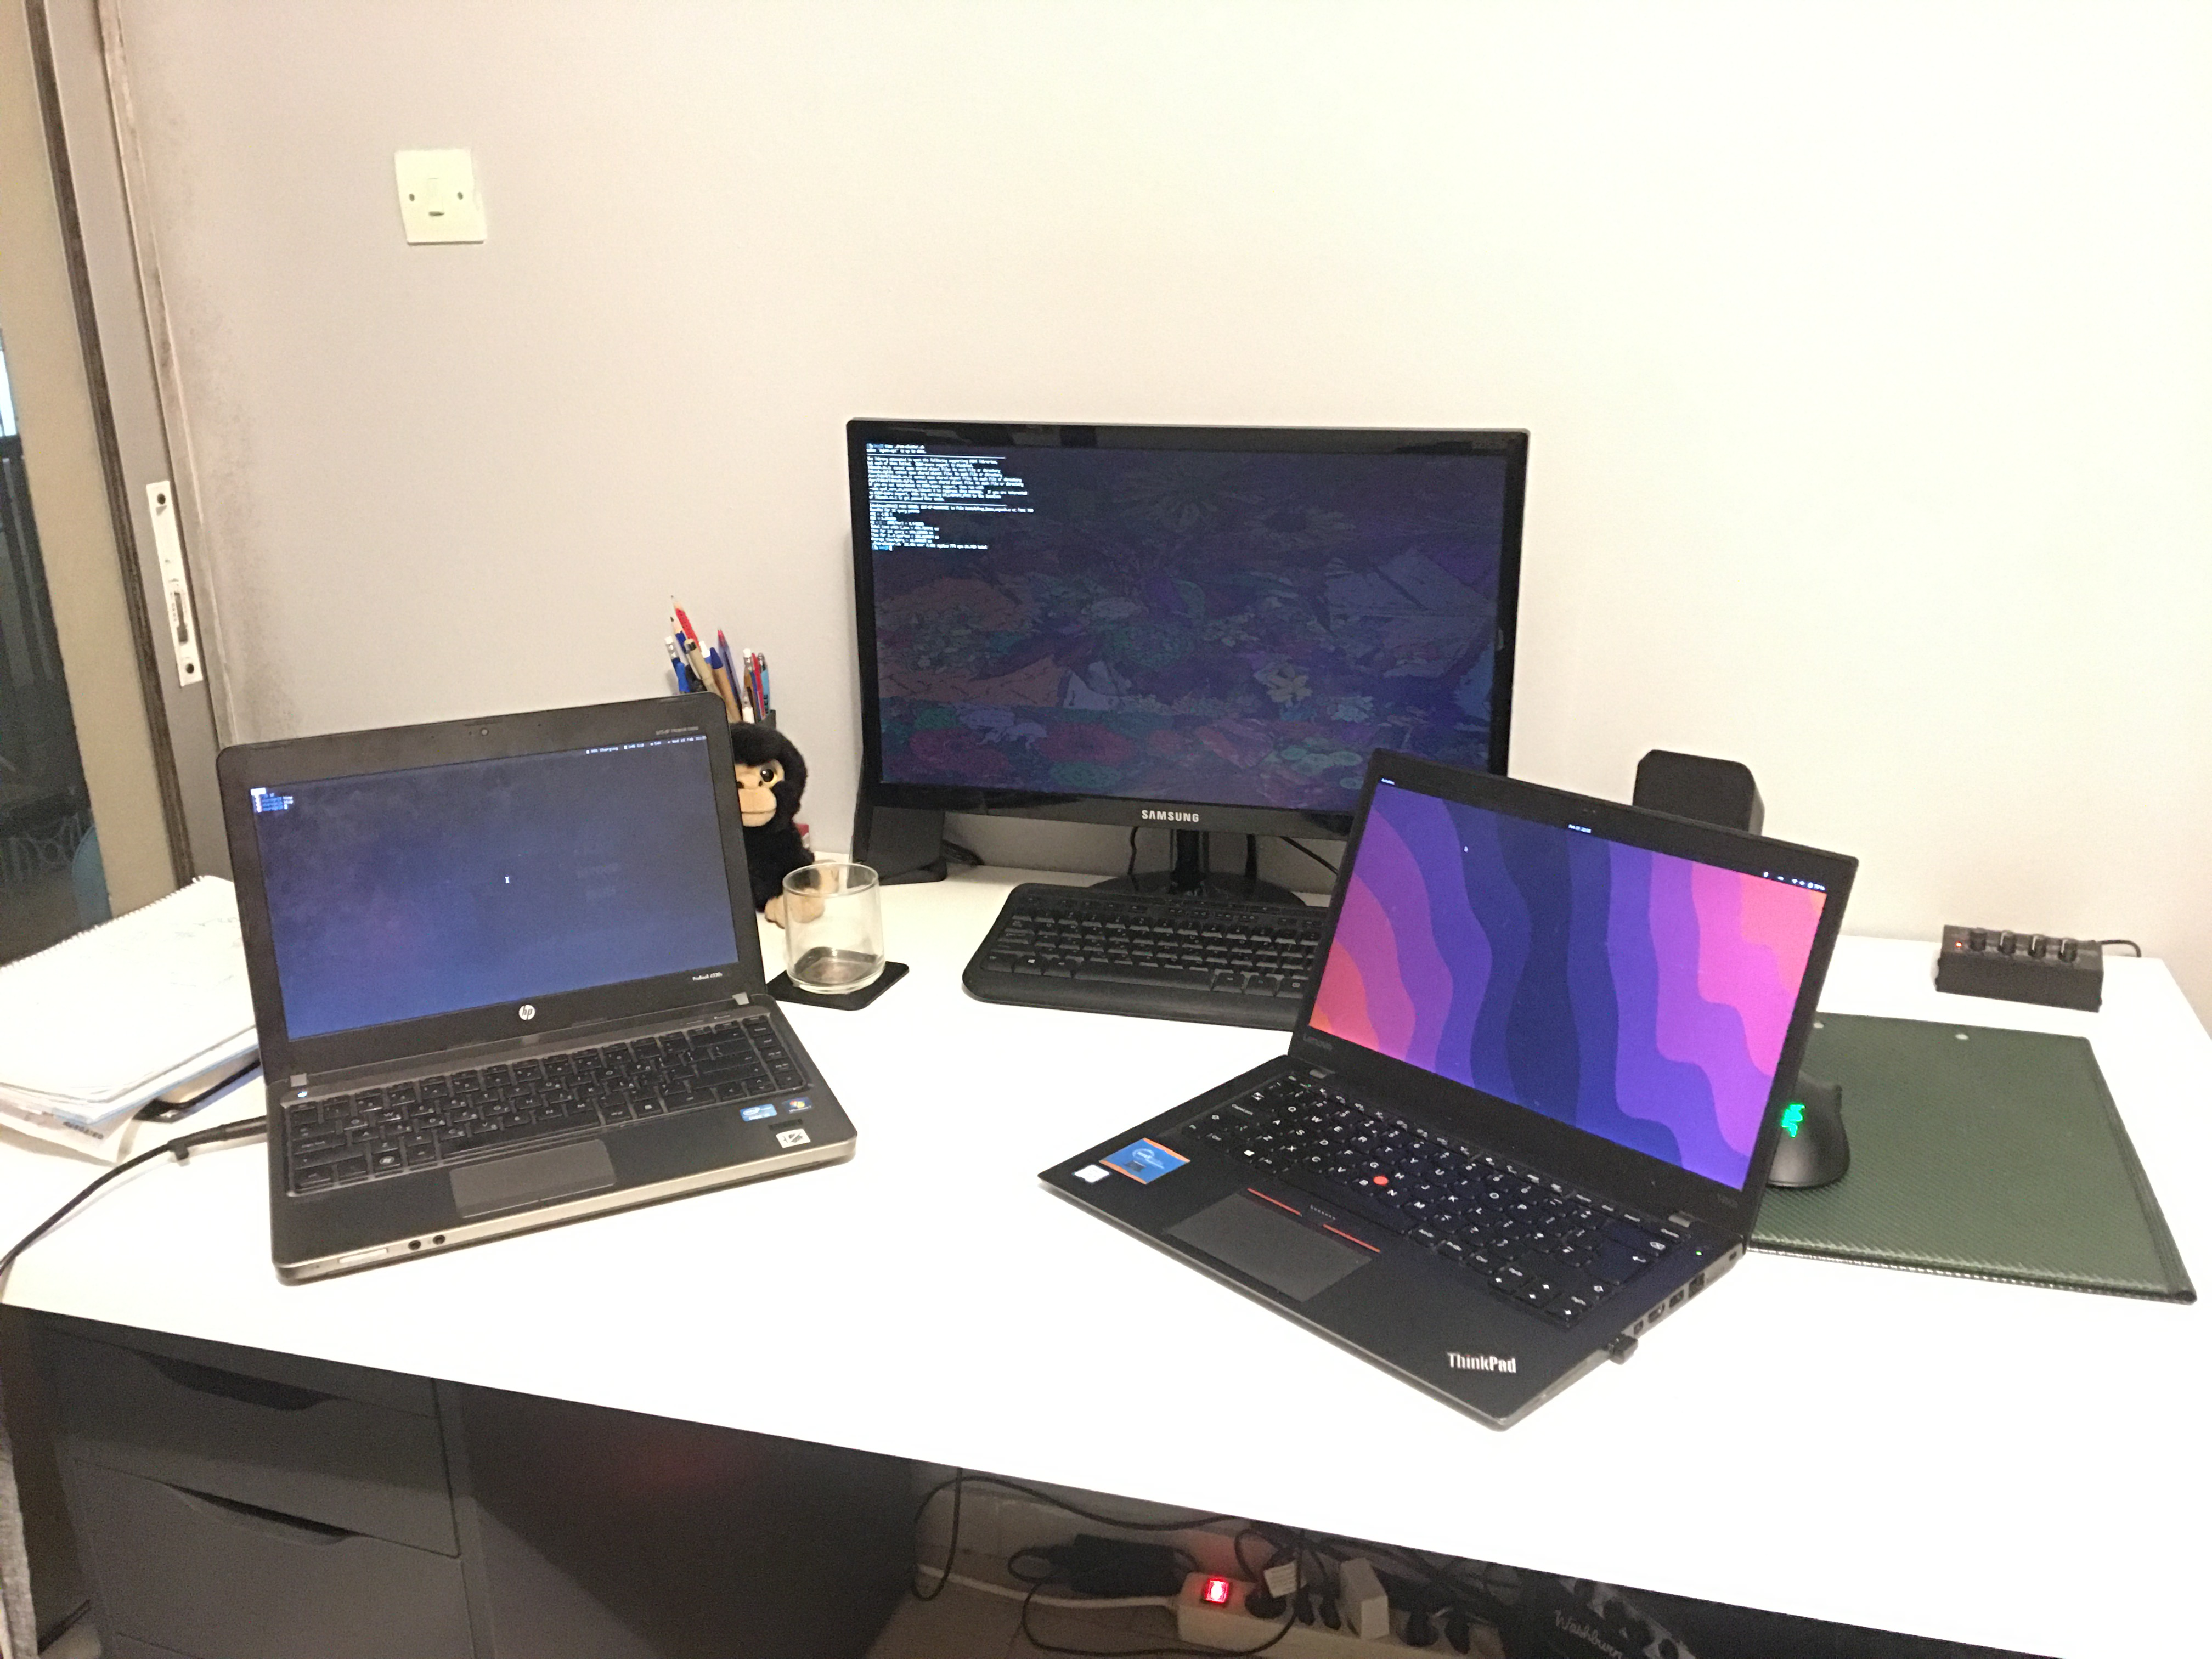
\includegraphics[width=0.7\textwidth]{assets/mpi_cluster.png}
    \end{center}
    \caption{Ο MPI Cluster μας να τρέχει τον αλγόριθμο K-NN σε ασύρματο LAN δίκτυο σε τρία μηχανήματα.}
    \label{fig:}
\end{figure}

Τα specifications των μηχανημάτων του cluster είναι: 

\begin{itemize}
    \item desktop: \src{Intel(R) Core(TM) i7-4770 CPU @ 3.40GHz}
    \item laptops: \src{Intel(R) Core(TM) i3-2310M CPU @ 2.10GHz} 
\end{itemize}

\subsubsection{Μετρήσεις}

\begin{figure}[H]
    \begin{center}
\begin{tikzpicture}
    \begin{axis}[
        xlabel={Αριθμός Queries},
        ylabel={Time (s)},
        xtick=data,
        xticklabels={32, 1024, 2048},
        ybar,
        enlarge x limits=0.15,
        bar width=10pt,
        legend style={at={(0.5,-0.20)}, anchor=north, legend columns=-1},
        legend entries={Serial, 3 Μηχανήματα},
        ymajorgrids=true,
        y grid style=dashed,
        nodes near coords,
        nodes near coords align={vertical},
        nodes near coords style={anchor=north},
        every node near coord/.append style={yshift=-2pt},
        every axis plot post/.append style={fill=blue!20},
        ]
        \addplot coordinates {(32, 4) (1024, 15) (2048, 28)};
        \addplot coordinates {(32, 9) (1024, 15) (2048, 24)};
    \end{axis}
\end{tikzpicture}
    \end{center}
    \caption{Χρόνοι εκτέλεσης της υλοποίησης με τον κώδικα MPI σε 3 Μηχανήματα (6 slots)}
    \label{fig:cluster_times}
\end{figure}

Ο συνολικός χρόνος εκτέλεσης πράγματι βελτιώνεται σε μεγάλο αριθμό queries αφού η μεταφορά δεδομένων μεταξύ των μηχανημάτων γίνεται μόνο
μετά τη λήξη εκτέλεσης του αλγορίθμου, πράγμα που κάνει το μεγάλο latency του δικτύου λιγότερο καταστροφικό στην ταχύτητα.
Ενδεχομένως να είχαμε περαιτέρω βελτίωση τα συστήματα επικοινωνούσαν μεταξύ τους με ethernet υψηλής ταχύτητας. \cite{mpi-ethernet}





\begin{figure}[H]
    \begin{center}
        \begin{subfigure}[b]{0.5\textwidth}
\begin{tikzpicture}
    \begin{axis}[
        xlabel={Αριθμός Διεργασιών},
        ylabel={Time/Query (ms)},
        xtick=data,
        xticklabels={1, 2, 4, 6, 8, 16},
        enlarge x limits=0.15,
        bar width=10pt,
        ymajorgrids=true,
        y grid style=dashed,
        nodes near coords,
        nodes near coords align={vertical},
        nodes near coords style={anchor=north},
        every node near coord/.append style={yshift=-2pt},
        ]
        \addplot coordinates {(1 , 9.03) (2 , 4.38) (4 , 3.39) (6 , 3.52) (8 , 3.63) (16, 3.6)};
    \end{axis}
\end{tikzpicture}
            \caption{Time}
        \end{subfigure}
        \begin{subfigure}[b]{0.5\textwidth}
\begin{tikzpicture}
    \begin{axis}[
        xlabel={Αριθμός Διεργασιών},
        ylabel={Time/Query Speedup},
        xtick=data,
        xticklabels={1, 2, 4, 6, 8, 16},
        enlarge x limits=0.15,
        bar width=10pt,
        ymajorgrids=true,
        y grid style=dashed,
        nodes near coords,
        nodes near coords align={vertical},
        nodes near coords style={anchor=north},
        every node near coord/.append style={},
        ]
        \addplot coordinates {(1, 1.00) (2, 2.06) (4, 2.66) (6, 2.56) (8, 2.48) (16, 2.50)};
    \end{axis}
\end{tikzpicture}
            \caption{Speedup}
        \end{subfigure}
    \end{center}
    \caption{Μετρήσεις για την υλοποίηση MPI σε ένα μηχάνημα.}
    \label{fig:mpi}
\end{figure}

Με την υλοποίηση του MPI φτάνουμε σε επιτάχυνση της τάξης \textbf{2.5x}.

\section{Έλεγχος Αποτελεσμάτων}

Για τον έλεγχο αποτελεσμάτων βασιστήκαμε στις μετρήσεις που εμφανίζονται με την εκτέλεση του προγράμματος.
Στον παρακάτω πίνακα παραθέτουμε τις μετρήσεις με την κάθε υλοποίηση.



\begin{table}[H]
    \centering
    \begin{tabular}{|l|c|c|c|c|c|}
    \hline
        Implementation & APE   & MSE   & $R^2$ \\ \hline
        Serial         & 4.79\% & 1.761781 & 0.922719 \\
        OpenMP         & 4.79\% & 1.761781 & 0.922719 \\
        OpenACC        & 4.79\% & 1.761781 & 0.922719 \\
        MPI            & 4.79\% & 1.761781 & 0.922719 \\
        CUDA           & 4.79\% & 1.761781 & 0.922719 \\
    \hline
    \end{tabular}
    \caption{Έλεγχος ορθότητας των αποτελεσμάτων. (1024 σημεία)}
\end{table}

Βλέπουμε πως όλα τα αποτελέσματα είναι ίδια με την υλοποίηση σε σειριακό κώδικα, οπότε η υλοποίηση μας είναι ορθή.

\bibliography{bibliography}

\end{document}
